\documentclass[11pt,aspectratio=169]{beamer}

\usepackage[utf8]{inputenc}
\usepackage[T1]{fontenc}
\usepackage[italian]{babel}
\usepackage{graphicx}
\usepackage{minted}
\usepackage{courier}
\renewcommand*\familydefault{\ttdefault}

\usepackage{fontawesome5}
\usepackage{tcolorbox}
\tcbuselibrary{skins}

\newtcolorbox{card}[2]{
    enhanced, colback=white, colframe=red_unipd,
    boxrule=1pt, arc=3pt,
    top=4pt, bottom=4pt, left=6pt, right=6pt,
    fonttitle=\bfseries\small,
    title={\faIcon{#1}~~#2}
}

\usetheme[pageofpages=of]{Unipd}

\title[Middleware Spring per Enrichment Dati]{Sviluppo di un Middleware basato su Spring per l'Arricchimento di Dati}
\author{Leonardo Baldo}
\institute[Univ. di Padova]{Università degli Studi di Padova\\Relatore: Prof. Marco Zanella}
\date{21 Settembre 2026}

\begin{document}

% ----------
\begin{frame}
    \titlepage
\end{frame}

% ----------
\begin{frame}{L'azienda}
    \begin{columns}[c]
        \column{0.60\textwidth}
        \begin{itemize}
            \setlength\itemsep{12pt}
            \item Stage presso \textbf{SyncLab S.r.l.}
            \item Soluzioni informatiche, ricerca e sviluppo, \textit{system integrator}
            \item Progetto: studio \textbf{Middleware} per l'arricchimento di dati
        \end{itemize}
        \column{0.30\textwidth}
        \begin{center}
            
\includegraphics[width=0.90\textwidth]{../assets/synclab.png}
        \end{center}
    \end{columns}
\end{frame}

% ----------
\begin{frame}{Perché serve un Middleware?}
    \begin{columns}[c]
        \column{0.5\textwidth}
        \begin{center}
            \textbf{Problema}
        \end{center}
        \vspace{6pt}
        \begin{itemize}
            \setlength\itemsep{12pt}
            \item \textbf{Connessioni} dirette con ogni sistema
            \item Ognuno deve \textbf{conoscere} il formato dati dell'altro
        \end{itemize}

        \vspace{12pt}
        \centering
        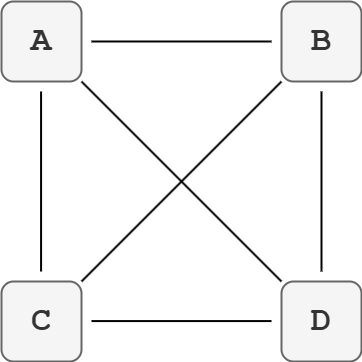
\includegraphics[width=0.25\textwidth]{../assets/middlewareSenza.drawio.png} \\
        {\scriptsize \textbf{Senza Middleware}}

        \column{0.5\textwidth}
        \begin{center}
            \textbf{Soluzione}
        \end{center}
        \vspace{6pt}
        \begin{itemize}
            \setlength\itemsep{12pt}
            \item Sistemi \textbf{eterogenei} che non comunicano direttamente
            \item \textbf{Disaccoppiamento} tra produttori e consumatori
        \end{itemize}

        \vspace{12pt}
        \centering
        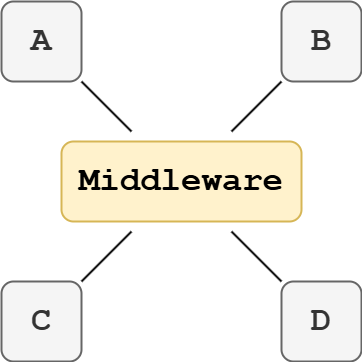
\includegraphics[width=0.25\textwidth]{../assets/middlewareCon.drawio.png} \\
        {\scriptsize \textbf{Con Middleware}}
    \end{columns}
\end{frame}

% ----------
\begin{frame}{Pattern architetturali}
    \begin{center}
        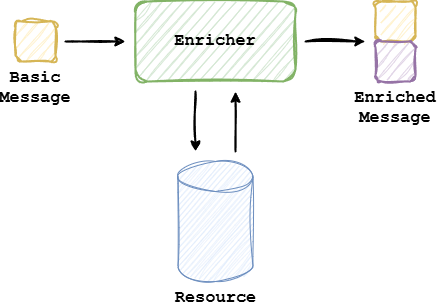
\includegraphics[width=0.50\textwidth]{../assets/contentEnricher.drawio.png}\\[4pt]
        \textbf{Content Enricher}: arricchisce il messaggio
    \end{center}
    % NOTE
    \note[item]{Dal punto di vista architetturale, il Middleware implementa un pattern noto come Content Enricher, uno degli Enterprise Integration Patterns: un catalogo di soluzioni standard per problemi ricorrenti nell'integrazione tra sistemi.}
    \note[item]{Il Content Enricher riceve in ingresso un messaggio con informazioni parziali, lo arricchisce interrogando una fonte dati esterna (come per esempio un database), e produce in uscita un messaggio completo.}
\end{frame}

% ----------
\begin{frame}{Pattern architetturali}
    \begin{center}
        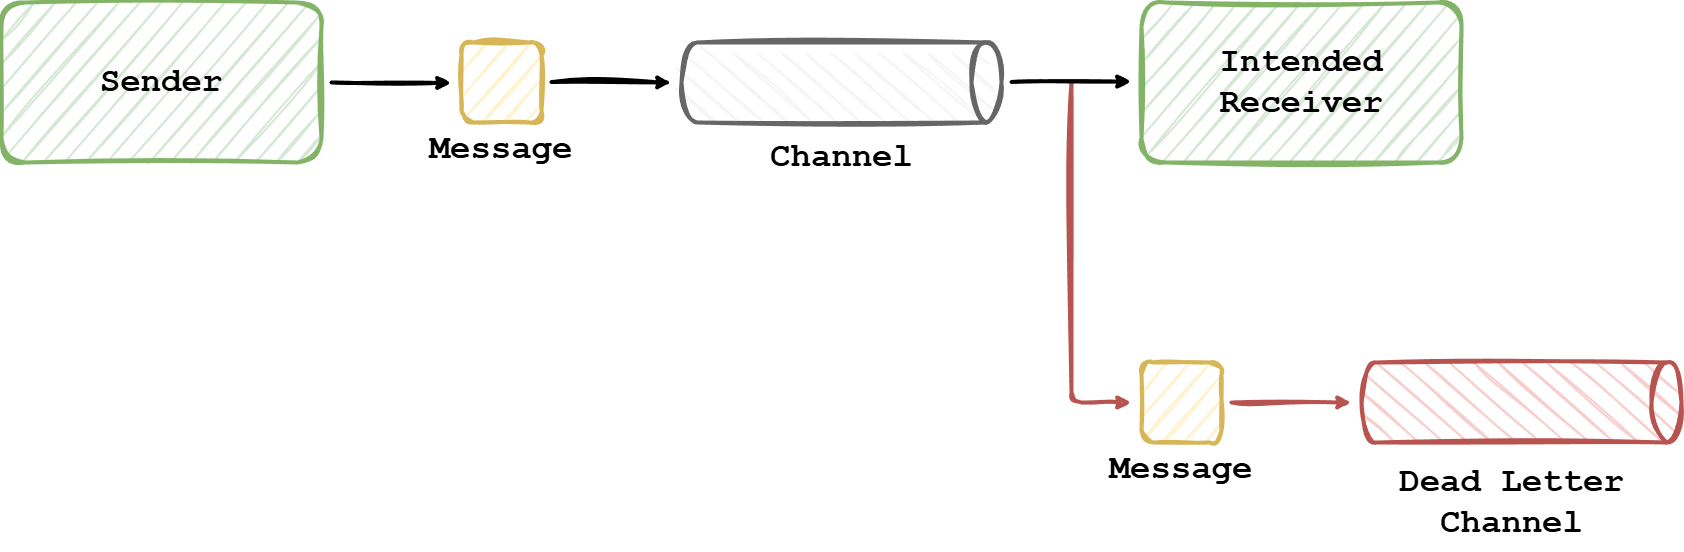
\includegraphics[width=0.80\textwidth]{../assets/deadLetterChannel.drawio.png}\\[4pt]
        \textbf{Dead Letter Channel}: isola gli errori
    \end{center}
\end{frame}

% ----------
\begin{frame}{Stack tecnologico}
    \begin{columns}[c]
        \column{0.3\textwidth}
        \centering
        \parbox[t][2.4em][t]{\linewidth}{\centering\scriptsize\textbf{Linguaggio e piattaforma}} \\[12pt]
        
\includegraphics[width=0.35\textwidth]{../assets/java.png} \\[16pt]
        
\includegraphics[width=0.75\textwidth]{../assets/apacheMaven.png}

        \column{0.3\textwidth}
        \centering
        \parbox[t][2.4em][t]{\linewidth}{\centering\scriptsize\textbf{Framework applicativo}} \\[12pt]
        
\includegraphics[width=0.90\textwidth]{../assets/spring.png}

        \column{0.3\textwidth}
        \centering
        \parbox[t][2.4em][t]{\linewidth}{\centering\scriptsize\textbf{Infrastruttura di supporto}} \\[12pt]
        
\includegraphics[width=0.75\textwidth]{../assets/docker.png} \\[16pt]
        
\includegraphics[width=0.35\textwidth]{../assets/postgresql.png} \\[16pt]
        
\includegraphics[width=0.70\textwidth]{../assets/apacheKafka.png}
    \end{columns}
\end{frame}

% ----------
\begin{frame}{Il progetto}
    \begin{center}
        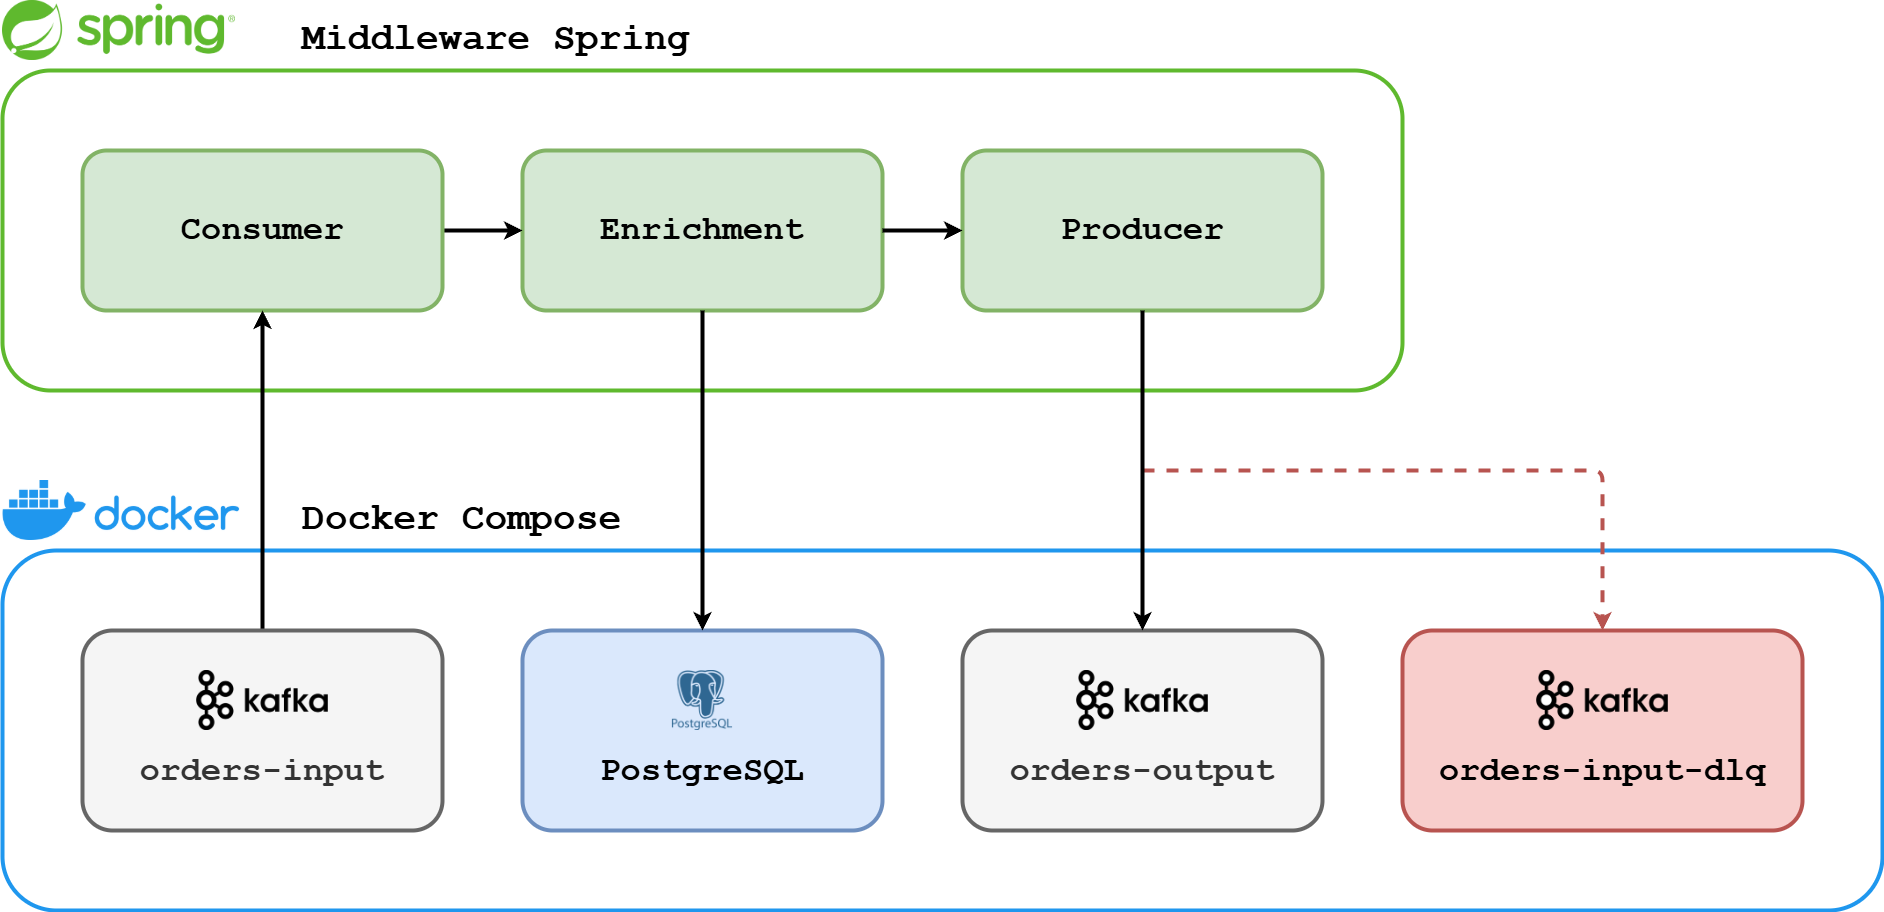
\includegraphics[width=0.75\textwidth]{../assets/progetto.drawio.png}
    \end{center}
\end{frame}

% ----------
\begin{frame}[fragile]{Implementazione - un esempio}
    \begin{columns}[c]
        \column{0.40\textwidth}
        Jakarta Persistence:
        \vspace{6pt}
        \begin{itemize}
            \setlength\itemsep{10pt}
            \item \textbf{@Entity} 
            \item \textbf{@Table}, \textbf{@Id}, \textbf{@Column}
        \end{itemize}
        \vspace{12pt}
        Lombok:
        \vspace{6pt}
        \begin{itemize}
            \setlength\itemsep{10pt}
            \item \textbf{@Getter}, \textbf{@Setter} 
            \item \textbf{@NoArgsConstructor} 
            \item \textbf{@AllArgsConstructor} 
        \end{itemize}
        \column{0.45\textwidth}
        \footnotesize
        \begin{minted}[fontsize=\scriptsize,frame=single,framesep=10pt]{java}
@Entity
@Table(name = "customers")
@Getter
@Setter
@NoArgsConstructor
@AllArgsConstructor
public class Customer {
    @Id
    private Long id;
    @Column(name = "full_name", 
        nullable = false)
    private String fullName;
    @Column(name = "email")
    private String email;
    @Column(name = "city")
    private String city;
}
        \end{minted}
    \end{columns}
\end{frame}

% ----------
\begin{frame}{Ambiente di sviluppo}
    \begin{columns}[c]
        \column{0.70\textwidth}
        \textbf{Docker}: Topic Kafka, PostgreSQL, Kafka UI \\
        \vspace{12pt}
        Le \textbf{partizioni} permettono letture e scritture in parallelo sullo stesso topic \\
        \vspace{12pt}
        \begin{center}
            \begin{tabular}{|l|c|l|}
                \hline
                \textbf{Topic} & \textbf{Partizioni} & \textbf{Ruolo} \\
                \hline
                orders-input & 3 & ingresso \\
                orders-output & 3 & uscita \\
                orders-input-dlq & 1 & errori \\
                \hline
            \end{tabular}
        \end{center}
        \column{0.25\textwidth}
        \begin{center}
            
\includegraphics[width=0.80\textwidth]{../assets/topic.png}
        \end{center}
    \end{columns}
\end{frame}

% ----------
\begin{frame}{Vantaggi ottenuti}
    \begin{columns}[t]
        \column{0.5\textwidth}
        \begin{center}
            {\Large\textcolor{red_unipd}{\faIcon{unlink}}}\\[4pt]
            \textbf{Disaccoppiamento}\\
            \small Sistemi indipendenti, \\facilmente modificabili
        \end{center}
        \vspace{14pt}
        \begin{center}
            {\Large\textcolor{red_unipd}{\faIcon{shield-alt}}}\\[4pt]
            \textbf{Nessuna perdita dati}\\
            \small Persistenza garantita da Kafka
        \end{center}
        \column{0.5\textwidth}
        \begin{center}
            {\Large\textcolor{red_unipd}{\faIcon{ban}}}\\[4pt]
            \textbf{Errori isolati}\\
            \small Gestiti tramite \\Dead Letter Channel
        \end{center}
        \vspace{14pt}
        \begin{center}
            {\Large\textcolor{red_unipd}{\faIcon{sync-alt}}}\\[4pt]
            \textbf{Ambiente riproducibile}\\
            \small Docker Compose, \\un solo comando
        \end{center}
    \end{columns}
\end{frame}

% ----------
\begin{frame}{Sviluppi futuri}
    \begin{columns}[c]
        \column{0.62\textwidth}
        \begin{itemize}
            \setlength\itemsep{20pt}
            \item \textbf{Apache Flink}: confronto già studiato a livello teorico
            \item \textbf{Test di performance}: metodologia di valutazione già definita, ma non eseguita
        \end{itemize}
        \column{0.30\textwidth}
        \centering
        
\includegraphics[width=0.7\textwidth]{../assets/ApacheFlink.png} \\
        \vspace{24pt}
        {\huge\textcolor{red_unipd}{\faIcon{tachometer-alt}}}
        {\huge\textcolor{red_unipd}{\faIcon{stopwatch}}}
        {\huge\textcolor{red_unipd}{\faIcon{hourglass-half}}}
        {\huge\textcolor{red_unipd}{\faIcon{database}}}
    \end{columns}
\end{frame}

% ----------
\begin{frame}{Sviluppi futuri}
    \begin{columns}[t]
        \column{0.5\textwidth}
        \begin{center}
            {\Large\textcolor{red_unipd}{\faIcon{tachometer-alt}}}\\[4pt]
            \textbf{Throughput}\\
            \small Messaggi arricchiti \\per secondo
        \end{center}
        \vspace{14pt}
        \begin{center}
            {\Large\textcolor{red_unipd}{\faIcon{stopwatch}}}\\[4pt]
            \textbf{Latenza end-to-end}\\
            \small Tempo tra evento grezzo e arricchito
        \end{center}
        \column{0.5\textwidth}
        \begin{center}
            {\Large\textcolor{red_unipd}{\faIcon{hourglass-half}}}\\[4pt]
            \textbf{Consumer lag}\\
            \small Quanto il sistema \\"sta al passo"
        \end{center}
        \vspace{14pt}
        \begin{center}
            {\Large\textcolor{red_unipd}{\faIcon{database}}}\\[4pt]
            \textbf{Costo interrogazione}\\
            \small Tempo di risposta \\della fonte dati
        \end{center}
    \end{columns}
\end{frame}

% ----------
\begin{frame}
    \begin{center}
        {\Huge \textbf{Grazie per l'attenzione}}\\[25pt]
        {\Large Domande?}
    \end{center}
\end{frame}

\end{document}